\section{Thực nghiệm SAT trên hai lượt main\_r1}
\subsection{Nguồn dữ liệu và kiểm tra tính đầy đủ}
Kết quả chính của bản thảo này lấy từ hai lượt chạy đã hoàn tất:
\begin{itemize}
\item \path{results/runs/cycles_main_r1.csv}: $C_n$ với
$\CycleFirst\leq n\leq\CycleLast$, gồm \CycleCount{} đồ thị;
\item \path{results/runs/products_main_r1.csv}: bảy họ product với
$\ProductFirst\leq n\leq\ProductLast$ và
$\ProductMFirst\leq m\leq\ProductMLast$, gồm \ProductCount{} đồ thị.
\end{itemize}
Mỗi dòng là một cặp Baseline/Symmetry trên cùng đồ thị. Tổng cộng có
\ComparisonCount{} cặp, tương ứng \WitnessCount{} lượt chạy. Các CSV lịch sử
vẫn được giữ để đối chiếu nhưng không được ghép vào bảng hoặc hình thực
nghiệm dưới đây. Sweep Petersen lịch sử và các kết quả ILP cũ không phải
đối chứng của hai lượt này.

Mỗi CSV đi kèm manifest cấu hình/mã nguồn/môi trường và JSONL chứa nhãn
incumbent, cận dưới, lịch sử thử span, bộ đếm của các lần thử đã hoàn tất.
Script xuất bảng kiểm tra tập tên đồ thị đúng miền quét, không trùng hoặc
thiếu dòng, hai span của mọi cặp OPT/OPT bằng nhau, và witness khớp dòng CSV.
Tất cả \WitnessCount{} labeling được kiểm tra lại bằng cách duyệt cạnh và
đường đi hai bước. Đồng thời dựng lại hai CNF tại \texttt{Count\_Span} để
đối chiếu số biến, clause thô và clause sau rút gọn; bước này không gọi SAT.
Hash của CSV, manifest, witness và script xuất bảng được lưu trong
\path{paper/generated/sources.json}. Kiểm tra nhãn không phải kiểm tra độc
lập các kết luận UNSAT: nghiên cứu chưa xuất chứng thư DRAT/LRAT.

\subsection{Cấu hình và định nghĩa phép đo}
\begin{table}[H]
\centering\small% Generated from main runs; do not edit numbers manually.
\begin{tabular}{llrllr}
\toprule
Tập & Miền $n$ & Số cặp & Solver & Search & Budget (s) \\
\midrule
Chu trình & 3--50 & 48 & glucose & hybrid & 60 \\
Product & 3--10 & 448 & glucose & hybrid & 180 \\
\bottomrule
\end{tabular}

\caption{Cấu hình lấy từ manifest. Với product, miền $m$ là
$\ProductMFirst$--$\ProductMLast$; budget áp dụng cho từng cấu hình của từng đồ thị.}
\end{table}
Hai lượt dùng Python 3.13.7, NetworkX 3.6.1 và PySAT 1.9.dev15 trên môi trường
macOS 13.7.8 x86\_64 được ghi trong manifest. Chưa lưu đầy đủ thông tin CPU,
RAM hoặc tải nền nên không diễn giải các số đo như đặc tính độc lập với máy.
Tên tùy chọn \texttt{hybrid} được giữ để tương thích CLI; lựa chọn span hiện
là trung điểm của khoảng cận, tức tìm kiếm nhị phân, với solver mới ở mỗi
lần thử. Thứ tự Base/Sym luân phiên theo instance; cả hai lượt dùng
\texttt{order\_offset=0}.

Baseline và Symmetry dùng cùng encoder và tiền xử lý chung. Chỉ $C_n$ cố
định $f(0)=0$, kết hợp thứ tự hai lân cận qua phản xạ; thí nghiệm này chưa
phân tách riêng tác động của hai điều kiện đó. Product không cố định gốc.
Các họ ghi ``Không thêm'' dùng cùng mô hình ở cả hai lượt, đóng vai trò
quan sát biến thiên khi lặp, không phải một kỹ thuật phá đối xứng mới.

\texttt{Time\_*} tính toàn bộ preprocessing, khởi động tiến trình, xây CNF,
tìm kiếm, validation và cleanup. Deadline được áp dụng cho tiến trình tìm
kiếm; preprocessing/cleanup có thể làm runtime vượt nhẹ budget. Thời gian
dựng lại hai CNF để đo kích thước nằm ngoài hai runtime này. Thời gian
\texttt{Encoding\_Time} và \texttt{SAT\_Solve\_Time} chỉ cộng các lần thử đã
hoàn tất, không bao gồm mọi overhead.

\texttt{Count\_Span} là giá trị lớn hơn của hai span incumbent. Khi cả hai
lượt chứng minh cùng tối ưu, đây là span tối ưu; nếu chưa, đây chỉ là một
cận trên khả thi chung. \texttt{Clause\_Raw\_*} đếm sau thay hằng ở gốc và
trước tiền xử lý chung; \texttt{Clause\_*} đếm sau tiền xử lý, gồm unit giữ
lại. Số biến là số được cấp phát, không phải số chưa bị gán bởi lan truyền.
Đây là CNF đầu vào, không phải số clause sau preprocessing/học của backend.

\subsection{Phạm vi đã giải và các trường hợp chưa tối ưu}
\begin{table}[H]
\centering\small\setlength{\tabcolsep}{4pt}
% Generated from main runs; do not edit numbers manually.
\begin{tabular}{lrrrrl}
\toprule
Họ & Số cặp & OPT/OPT & Chưa tối ưu & Span (OPT) & Đối xứng \\
\midrule
$C_n$ & 48 & 48 & 0 & 4 & Gốc + thứ tự \\
$C_n \mathbin{\square} C_m$ & 64 & 62 & 2 & 6--8 & Thứ tự \\
$C_n \mathbin{\square} P_m$ & 64 & 64 & 0 & 6--7 & Thứ tự \\
$P_n \mathbin{\square} P_m$ & 64 & 64 & 0 & 6 & Không thêm \\
$C_n \circ C_m$ & 64 & 64 & 0 & 7--14 & Thứ tự \\
$C_n \circ P_m$ & 64 & 64 & 0 & 7--14 & Thứ tự \\
$P_n \circ C_m$ & 64 & 64 & 0 & 7--14 & Không thêm \\
$P_n \circ P_m$ & 64 & 64 & 0 & 6--14 & Không thêm \\
\bottomrule
\end{tabular}

\caption{Kết quả theo từng họ. Span chỉ tổng hợp các cặp OPT/OPT bằng nhau;
``Chưa tối ưu'' đếm cặp có ít nhất một lượt chưa xác nhận tối ưu.}
\end{table}
Có \PairedOpt{} cặp cùng OPT và không có cặp OPT/OPT nào bất đồng span.
Mọi chu trình trong miền khảo sát đạt span 4. Hai instance product chưa
xác nhận tối ưu ở cả hai cấu hình là $C_9\mathbin{\square}C_{10}$ và
$C_{10}\mathbin{\square}C_9$:
\begin{table}[H]
\centering\small% Generated from main runs; do not edit numbers manually.
\begin{tabular}{lrrrrr}
\toprule
Đồ thị & $L_B$ & $U_B$ & $L_S$ & $U_S$ & Span đếm \\
\midrule
$C_{9}\mathbin{\square}C_{10}$ & 5 & 10 & 5 & 10 & 10 \\
$C_{10}\mathbin{\square}C_{9}$ & 7 & 8 & 7 & 8 & 8 \\
\bottomrule
\end{tabular}

\caption{Khoảng cận $[L,U]$ ở các lượt FEASIBLE; $U$ có labeling cụ thể.
Các cận lấy từ witness, không suy từ một công thức chưa chứng minh.}
\end{table}
Hai đồ thị này đẳng cấu qua đổi tọa độ. Incumbent có thể khác nhau do thứ tự
đỉnh và lịch sử tìm kiếm; không coi hai cận trên đó là hai giá trị tối ưu.
Ở $C_9\mathbin{\square}C_{10}$, cả hai lượt bị ngắt trước khi có lần thử span
hoàn tất, nên bộ đếm đã ghi bằng 0 không có nghĩa solver không thực hiện
công việc. Cả bốn lượt FEASIBLE đều có \texttt{Stats\_Complete=False}.

\subsection{Kích thước CNF và thời gian theo từng họ}
Đặt $t_B,t_S$ là thời gian của hai cấu hình. Tỉ số $t_B/t_S>1$ cho biết
lượt Symmetry nhanh hơn trên cặp đó. Bảng dưới dùng riêng tập cặp cùng OPT;
các cặp FEASIBLE đã được báo riêng và không được gán runtime thay thế.
\begin{table}[H]
\centering\small% Generated from main runs; do not edit numbers manually.
\begin{tabular}{lrrrr}
\toprule
Họ & OPT/OPT & $\sum t_B$ (s) & $\sum t_S$ (s) & Trung vị $t_B/t_S$ \\
\midrule
$C_n$ & 48 & 22.987 & 23.983 & 1.000 \\
$C_n \mathbin{\square} C_m$ & 62 & 326.842 & 131.803 & 1.103 \\
$C_n \mathbin{\square} P_m$ & 64 & 39.972 & 38.580 & 1.021 \\
$P_n \mathbin{\square} P_m$ & 64 & 35.113 & 35.582 & 1.000 \\
$C_n \circ C_m$ & 64 & 769.385 & 447.613 & 1.120 \\
$C_n \circ P_m$ & 64 & 701.840 & 497.427 & 1.112 \\
$P_n \circ C_m$ & 64 & 402.675 & 402.658 & 0.992 \\
$P_n \circ P_m$ & 64 & 402.654 & 405.998 & 1.005 \\
\bottomrule
\end{tabular}

\caption{Tổng runtime và trung vị tỉ số trên các cặp cùng OPT. Tổng thời gian
và trung vị tỉ số là hai đại lượng khác nhau.}
\end{table}
\begin{table}[H]
\centering\small\setlength{\tabcolsep}{4pt}% Generated from main runs; do not edit numbers manually.
\begin{tabular}{lrrrrr}
\toprule
Họ & Giảm biến (\%) & Giảm clause (\%) & Giảm & Bằng & Tăng \\
\midrule
$C_n$ & 3.77 & 12.58 & 48 & 0 & 0 \\
$C_n \mathbin{\square} C_m$ & 0.00 & 0.83 & 62 & 0 & 0 \\
$C_n \mathbin{\square} P_m$ & 0.00 & 0.58 & 64 & 0 & 0 \\
$P_n \mathbin{\square} P_m$ & 0.00 & 0.00 & 0 & 64 & 0 \\
$C_n \circ C_m$ & 0.00 & 1.11 & 64 & 0 & 0 \\
$C_n \circ P_m$ & 0.00 & 1.14 & 64 & 0 & 0 \\
$P_n \circ C_m$ & 0.00 & 0.00 & 0 & 64 & 0 \\
$P_n \circ P_m$ & 0.00 & 0.00 & 0 & 64 & 0 \\
\bottomrule
\end{tabular}

\caption{Trung vị phần trăm giảm biến và clause; ba cột cuối đếm số cặp có
clause Symmetry giảm/bằng/tăng so với Baseline. Cùng tập cặp OPT/OPT như bảng thời gian.}
\end{table}
Với chu trình, trung vị giảm clause là \CycleClauseMedian\%, nhưng trung vị
$t_B/t_S$ chỉ là \CycleTimeRatio. Vì các instance nhỏ, chi phí khởi động và
phần ngoài lời gọi SAT đáng kể; dữ liệu một lượt này chưa cho thấy lợi ích
thời gian tổng rõ rệt từ việc giảm kích thước CNF.

Trên các cặp cùng OPT của $C_n\mathbin{\square}C_m$, trung vị tỉ số là
\CxCTimeRatio, trong khi tỉ số hai tổng thời gian là \CxCTotalTimeRatio.
Sự khác nhau cho thấy tổng thời gian chịu ảnh hưởng nhiều hơn bởi một số
instance tốn thời gian. Với $C_n\circ C_m$ và $C_n\circ P_m$, trung vị lần
lượt là \CoCTimeRatio{} và \CoPTimeRatio. Đây là cải thiện quan sát trong
lượt chạy này, chưa phải khẳng định ổn định qua nhiều lần lặp. Các họ
$P_n\mathbin{\square}P_m$, $P_n\circ P_m$, $P_n\circ C_m$ không thêm đối xứng
riêng; chênh lệch thời gian giữa hai lượt của chúng phản ánh biến thiên phép đo.

\begin{figure}[htbp]
\centering
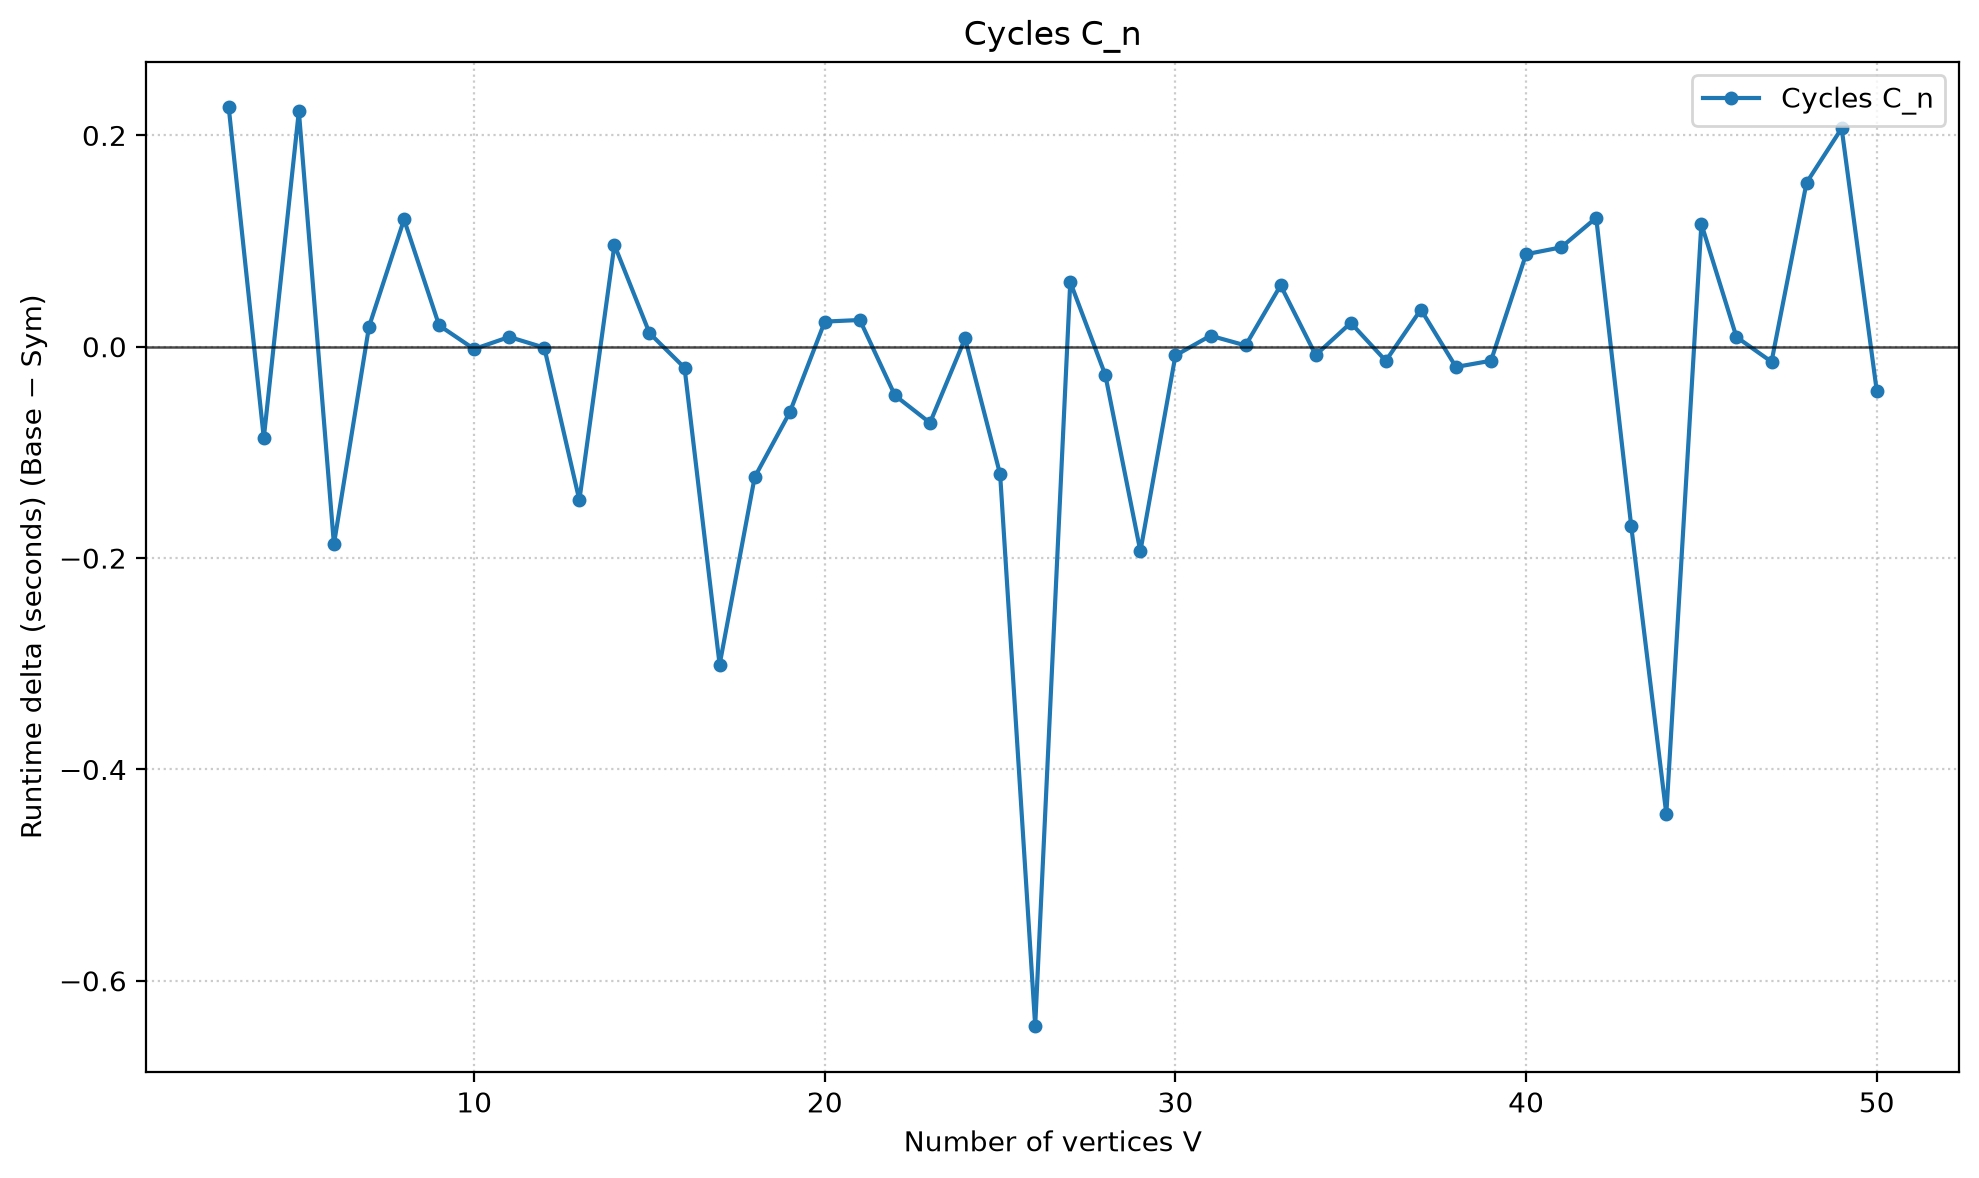
\includegraphics[width=0.49\linewidth]{paper/generated/cycles_main_r1_plots/delta_runtime_C.png}
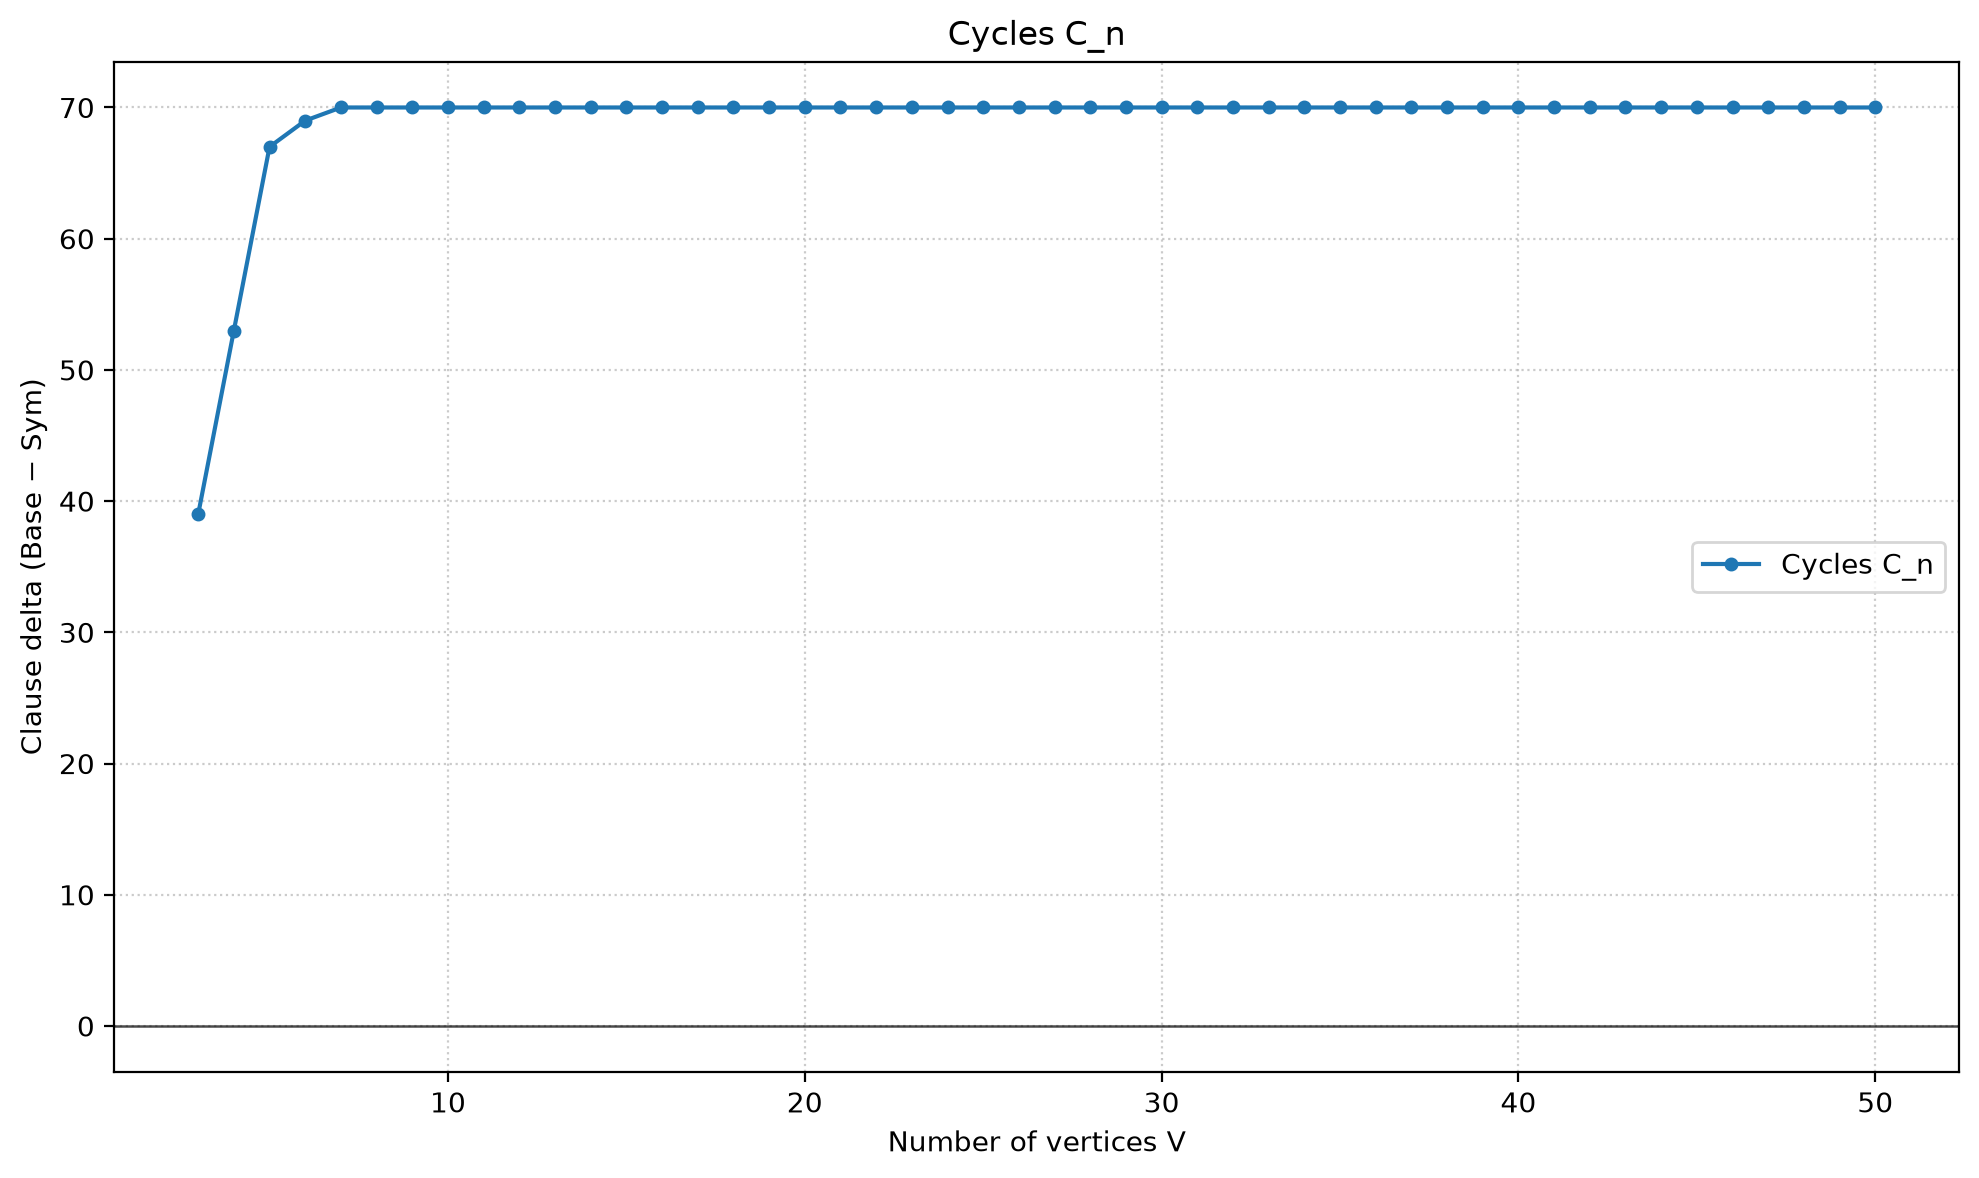
\includegraphics[width=0.49\linewidth]{paper/generated/cycles_main_r1_plots/delta_clauses_C.png}
\caption{Chu trình: chênh lệch runtime và số clause Base trừ Sym. Giá trị
âm ở hình thời gian nghĩa là lượt Symmetry chậm hơn.}
\end{figure}
\begin{figure}[htbp]
\centering
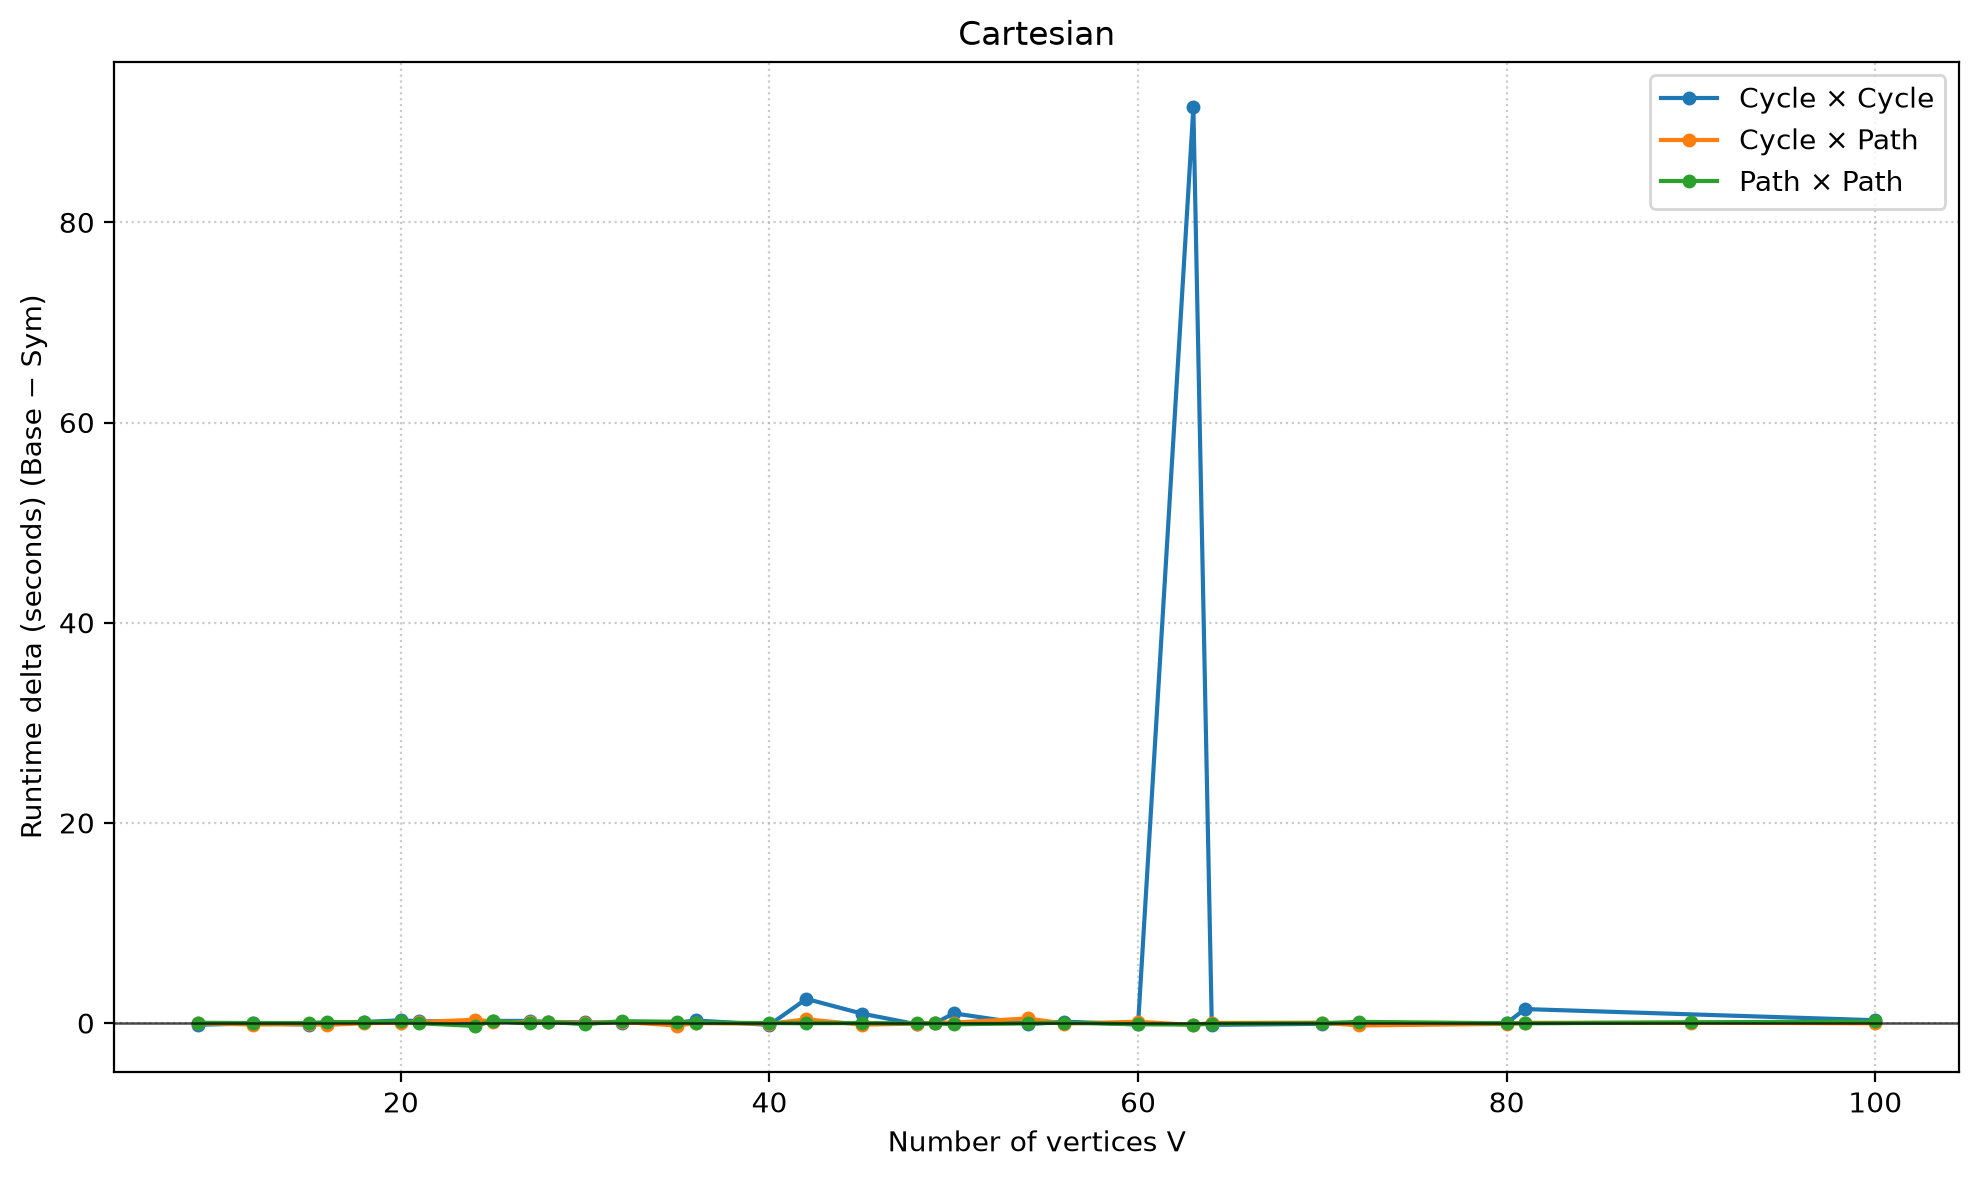
\includegraphics[width=0.49\linewidth]{paper/generated/products_main_r1_plots/delta_runtime_cartesian.png}
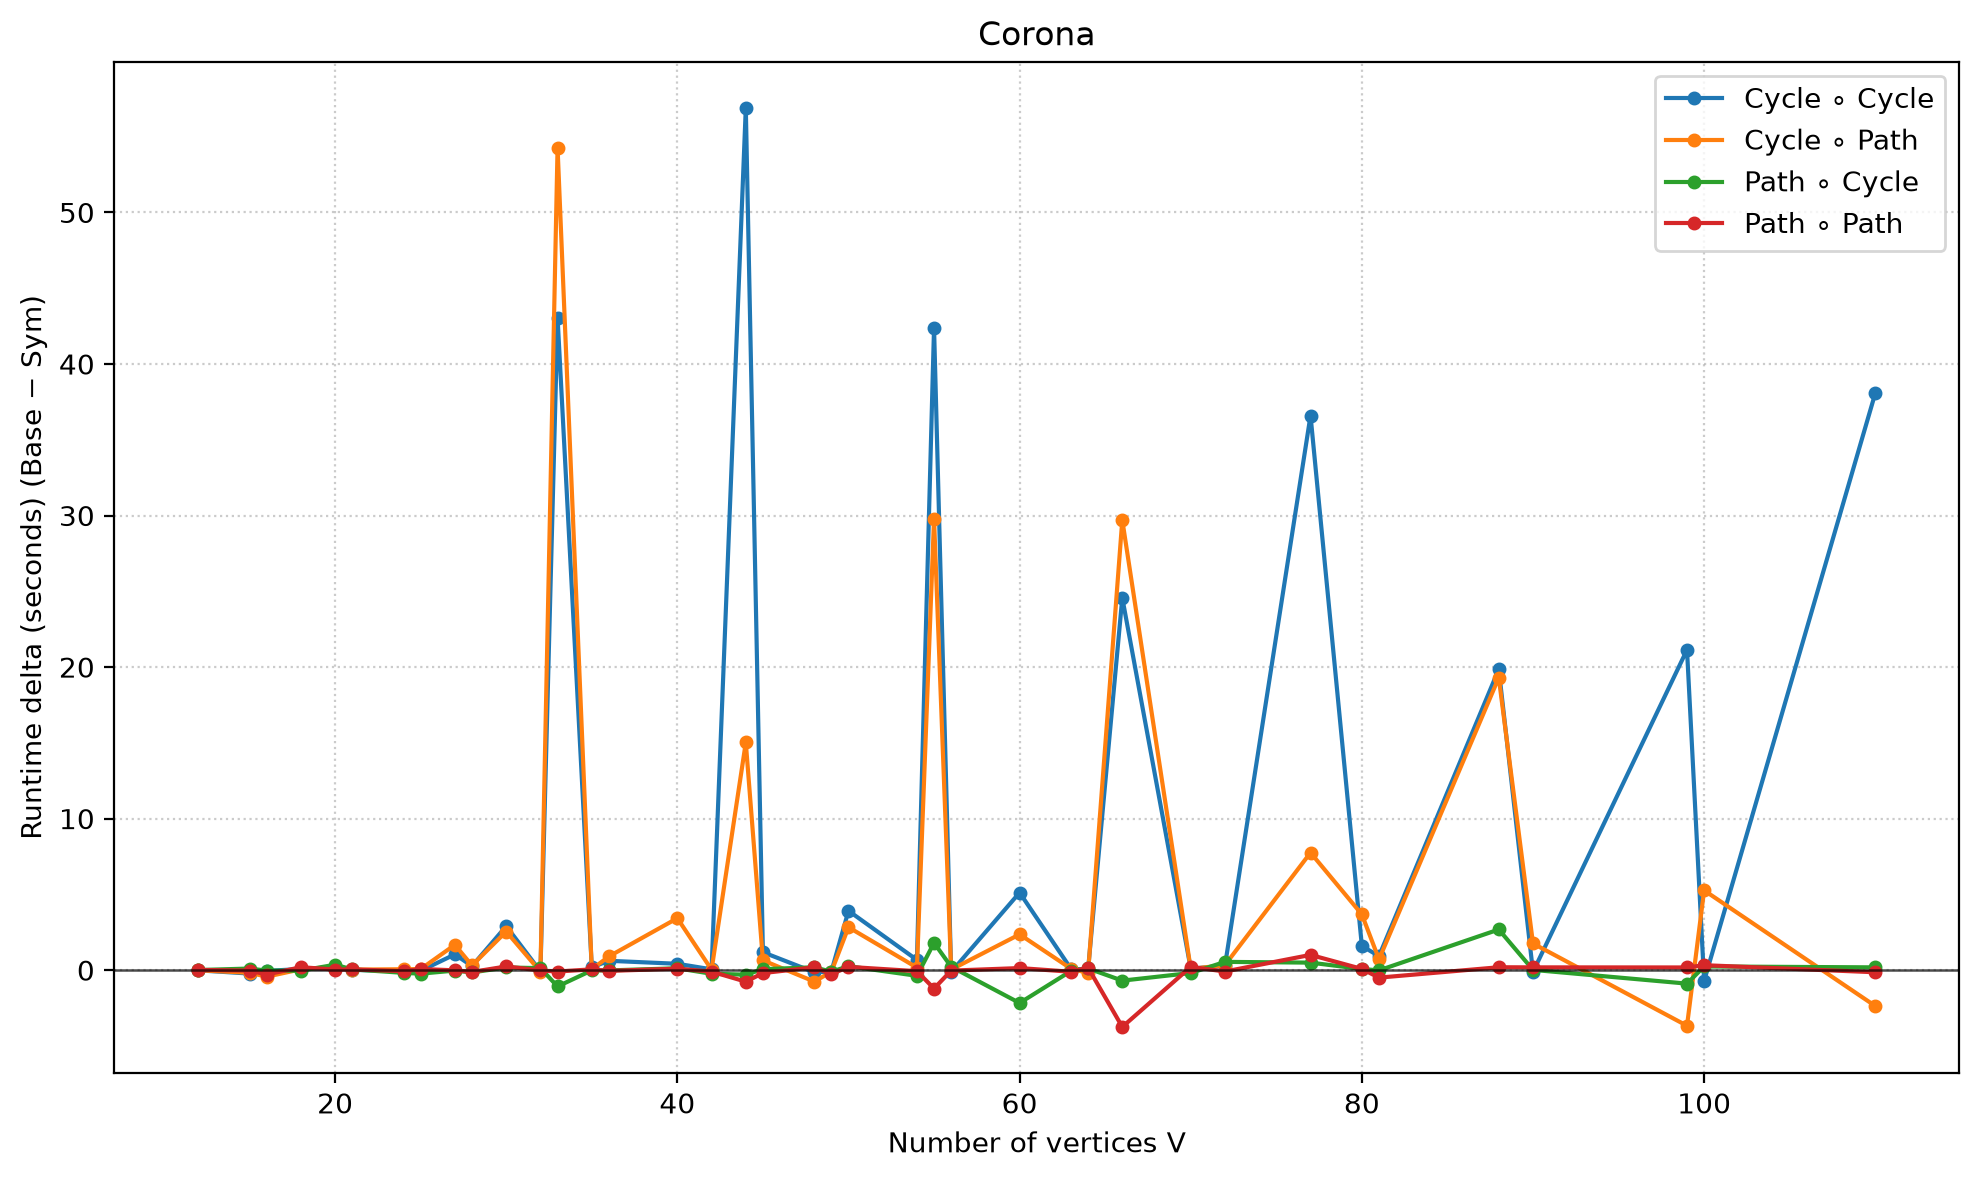
\includegraphics[width=0.49\linewidth]{paper/generated/products_main_r1_plots/delta_runtime_corona.png}
\caption{Runtime product: mỗi đường là một họ riêng, mỗi điểm là trung bình
chênh lệch trên các cặp cùng họ, cùng số đỉnh và cùng OPT. Không gộp các họ
thành một đường trung bình; hai cặp chưa tối ưu không nằm trong hình này.}
\end{figure}
\begin{figure}[htbp]
\centering
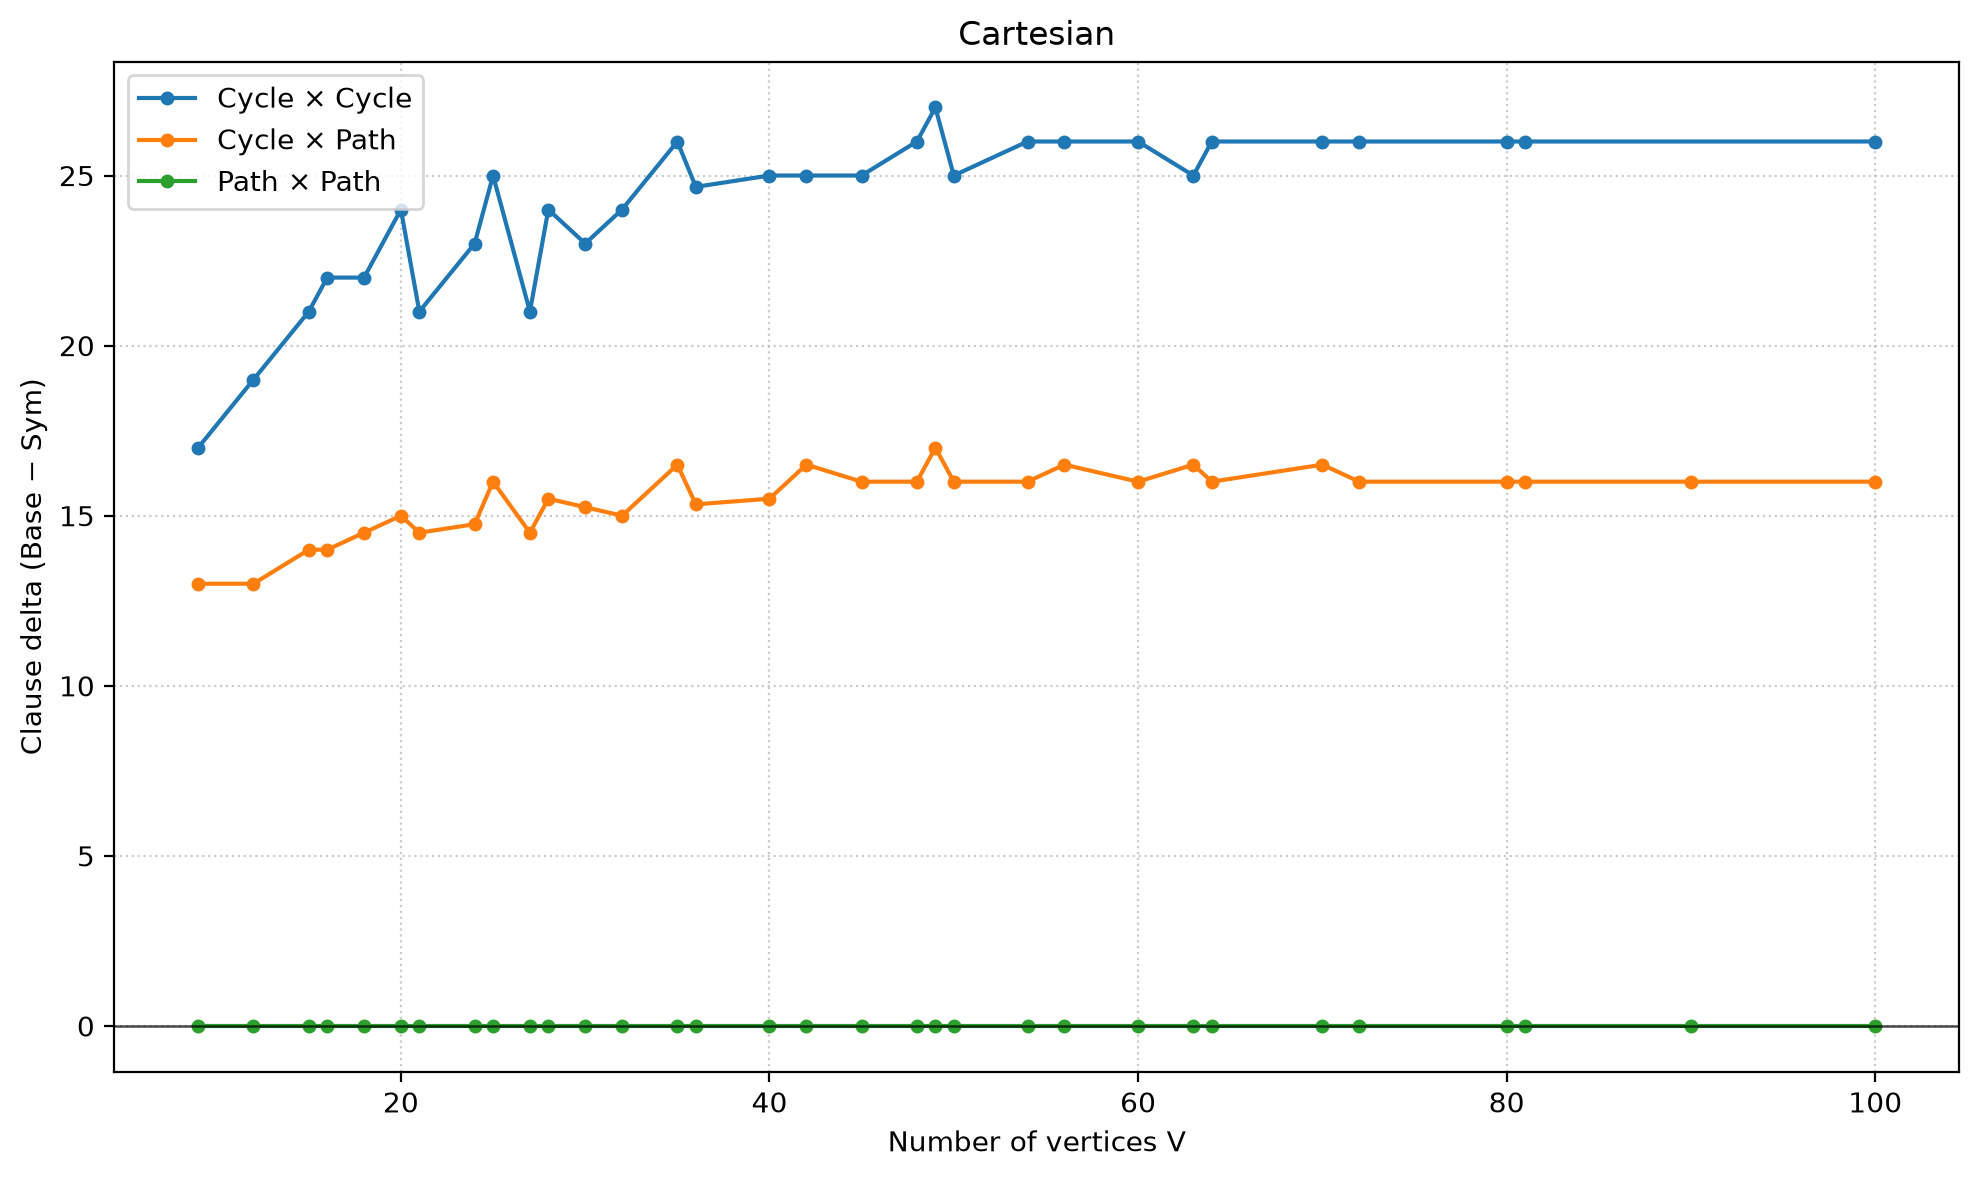
\includegraphics[width=0.49\linewidth]{paper/generated/products_main_r1_plots/delta_clauses_cartesian.png}
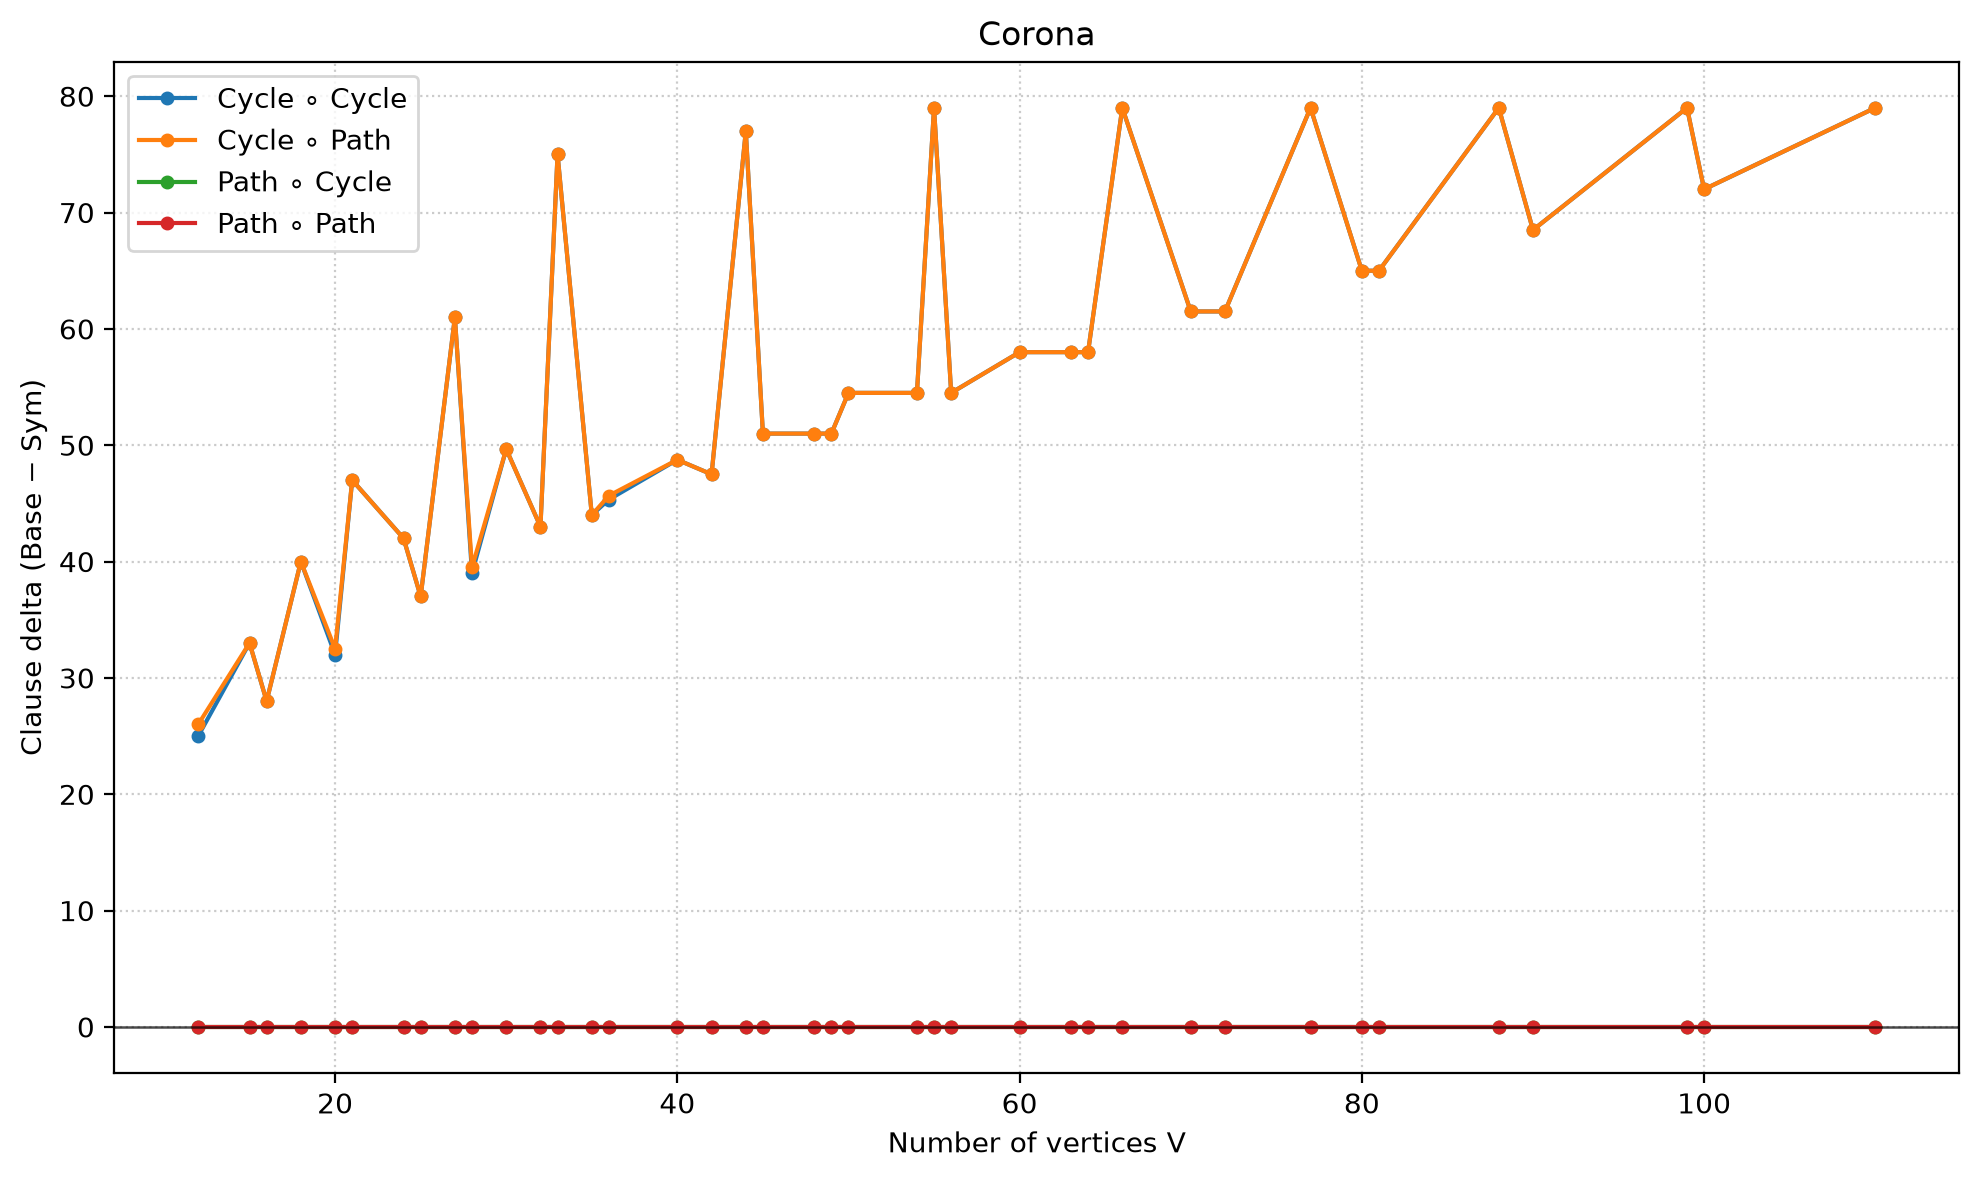
\includegraphics[width=0.49\linewidth]{paper/generated/products_main_r1_plots/delta_clauses_corona.png}
\caption{Clause product: Base trừ Sym tại cùng span, sau cùng tiền xử lý,
trên tập cặp OPT/OPT. Các đường giá trị 0 có thể trùng nhau ở những họ không
thêm điều kiện đối xứng riêng.}
\end{figure}
\FloatBarrier

\subsection{Bộ đếm tìm kiếm và thời gian thành phần}
\begin{table}[H]
\centering\small\setlength{\tabcolsep}{4pt}% Generated from main runs; do not edit numbers manually.
\begin{tabular}{lrrrr}
\toprule
Họ & Xung đột B & Xung đột S & Quyết định B & Quyết định S \\
\midrule
$C_n$ & 490 & 16 & 1014 & 304 \\
$C_n \mathbin{\square} C_m$ & 2822176 & 1561898 & 3703052 & 2086601 \\
$C_n \mathbin{\square} P_m$ & 62458 & 56542 & 96318 & 87201 \\
$P_n \mathbin{\square} P_m$ & 8282 & 8282 & 15175 & 15175 \\
$C_n \circ C_m$ & 28922138 & 19787058 & 35712056 & 24679416 \\
$C_n \circ P_m$ & 25550270 & 21037672 & 31640833 & 26452185 \\
$P_n \circ C_m$ & 15624199 & 15624199 & 19374024 & 19374024 \\
$P_n \circ P_m$ & 17120804 & 17120804 & 21294514 & 21294514 \\
\bottomrule
\end{tabular}

\caption{Tổng xung đột và quyết định của Glucose qua các lần thử span đã
hoàn tất, chỉ trên cặp OPT/OPT. Bao gồm cả lần thử SAT và UNSAT.}
\end{table}
\begin{table}[H]
\centering\small% Generated from main runs; do not edit numbers manually.
\begin{tabular}{lrrrr}
\toprule
Họ & Dựng CNF B & Dựng CNF S & SAT B & SAT S \\
\midrule
$C_n$ & 0.0033 & 0.0027 & 0.0001 & 0.0000 \\
$C_n \mathbin{\square} C_m$ & 0.0718 & 0.0652 & 0.0241 & 0.0143 \\
$C_n \mathbin{\square} P_m$ & 0.0551 & 0.0558 & 0.0076 & 0.0069 \\
$P_n \mathbin{\square} P_m$ & 0.0454 & 0.0443 & 0.0012 & 0.0011 \\
$C_n \circ C_m$ & 0.0661 & 0.0629 & 0.3988 & 0.2334 \\
$C_n \circ P_m$ & 0.0629 & 0.0605 & 0.4020 & 0.2809 \\
$P_n \circ C_m$ & 0.0642 & 0.0740 & 0.0628 & 0.0683 \\
$P_n \circ P_m$ & 0.0647 & 0.0531 & 0.0808 & 0.1007 \\
\bottomrule
\end{tabular}

\caption{Trung vị thời gian dựng CNF và thời gian bên trong lời gọi SAT
(giây), cộng theo từng quá trình tìm kiếm rồi lấy trung vị trên cặp OPT/OPT.}
\end{table}
Số clause ở một span chung đo kích thước mô hình; tổng quyết định/xung đột
đo công việc qua toàn bộ các span đã thử. Hai cấu hình có thể đi qua những
span khác nhau khi tìm được incumbent khác nhau; do đó không diễn giải
bộ đếm tổng thành hiệu năng của một lời gọi tại span cố định. Bộ đếm đầy đủ
ở các lượt OPT hỗ trợ phân tích tìm kiếm nhưng không tự thay thế phép đo
runtime hoặc các lượt lặp. Các bộ đếm khác backend cũng không được mặc
nhiên coi là cùng thước đo.

\subsection{Tái lập và giới hạn kiểm chứng}
Lệnh \texttt{make report} kiểm tra hai CSV cùng manifest/witness, dựng lại
counts, sinh bảng, sinh hình rồi biên dịch bản thảo. Các file kết quả gốc
không bị sửa. Resume của benchmark chỉ nhận cùng cấu hình, source, schema
và môi trường; muốn đổi budget hoặc thử lại dòng FEASIBLE phải tạo lượt mới.

Bộ kiểm thử dùng oracle vét cạn trên mọi đồ thị atlas đến 5 đỉnh, kiểm tra
mọi phép gán trên đồ thị 3 đỉnh, các giá trị $h,k$ ở mức encoder, tính tương
đương của rút gọn, phản xạ của các constructor và các ràng buộc ILP. Hai
kiểm thử tích hợp ILP chưa qua vì giới hạn runtime/license trong môi trường
kiểm tra. Vì vậy bản thảo này không đưa ra kết luận SAT nhanh hơn ILP.
Hai lượt main\_r1 là một lần đo mỗi cấu hình trên mỗi instance; chưa có
ước lượng phương sai hoặc khoảng tin cậy. Chọn riêng các cặp OPT/OPT có
thể thiên về instance dễ, nên các bảng thời gian không đại diện toàn bộ
miền khi vẫn còn cặp timeout.
